最適化の方法として,複数のパラメータからモデル,実行環境に即したパラメータを選択するという手法を選択したが,
そのためには複数のパラメータでシミュレーションを行いその結果を集約するプログラムが必要となる.\\
本研究ではこのパラメータ選択を容易かつ高速に行うため以下に示すプログラムを作成した.\\
・MODファイルからパラメータとなりうる変数を自動で抽出し,それぞれの関係性を元に配列とその順序の候補を生成する.\\
・ジョブキューのシステムを持っているマシンにおいて,複数のジョブを並行して投げ結果を非同期的に集約できる.\\
・実行結果を最適化前のデフォルトの結果と比較し,実行結果に対して影響がないかを確認する.\\
・json形式で実行するファイル,各パラメータの範囲(プロセス数は1から10など)を指定することができる.\\
\subsubsection{全体構成}
はじめにシミュレータプログラムを構成する要素について示す.\\
( TODO: 章番号)にあるアルゴリズムで述べたように,探索の対象となるパラメータは,モデルに依存するパラメータ,
実行マシンに依存するパラメータそしてコンパイルに関わるパラメータの3つに大別される.\\
そのうち,モデルとコンパイルに関わるパラメータは実行形式の生成に関与し,実行マシンに関わるパラメータは
ジョブスクリプトの生成に関わる.\\
\paragraph{単一ジョブの実行}
パラメータのシミュレーションを一度行う際のプログラムの動作を次に示す.\\
\begin{figure}[htb]
% h:here, t:top, b:bottom, p:page
  \begin{center}
    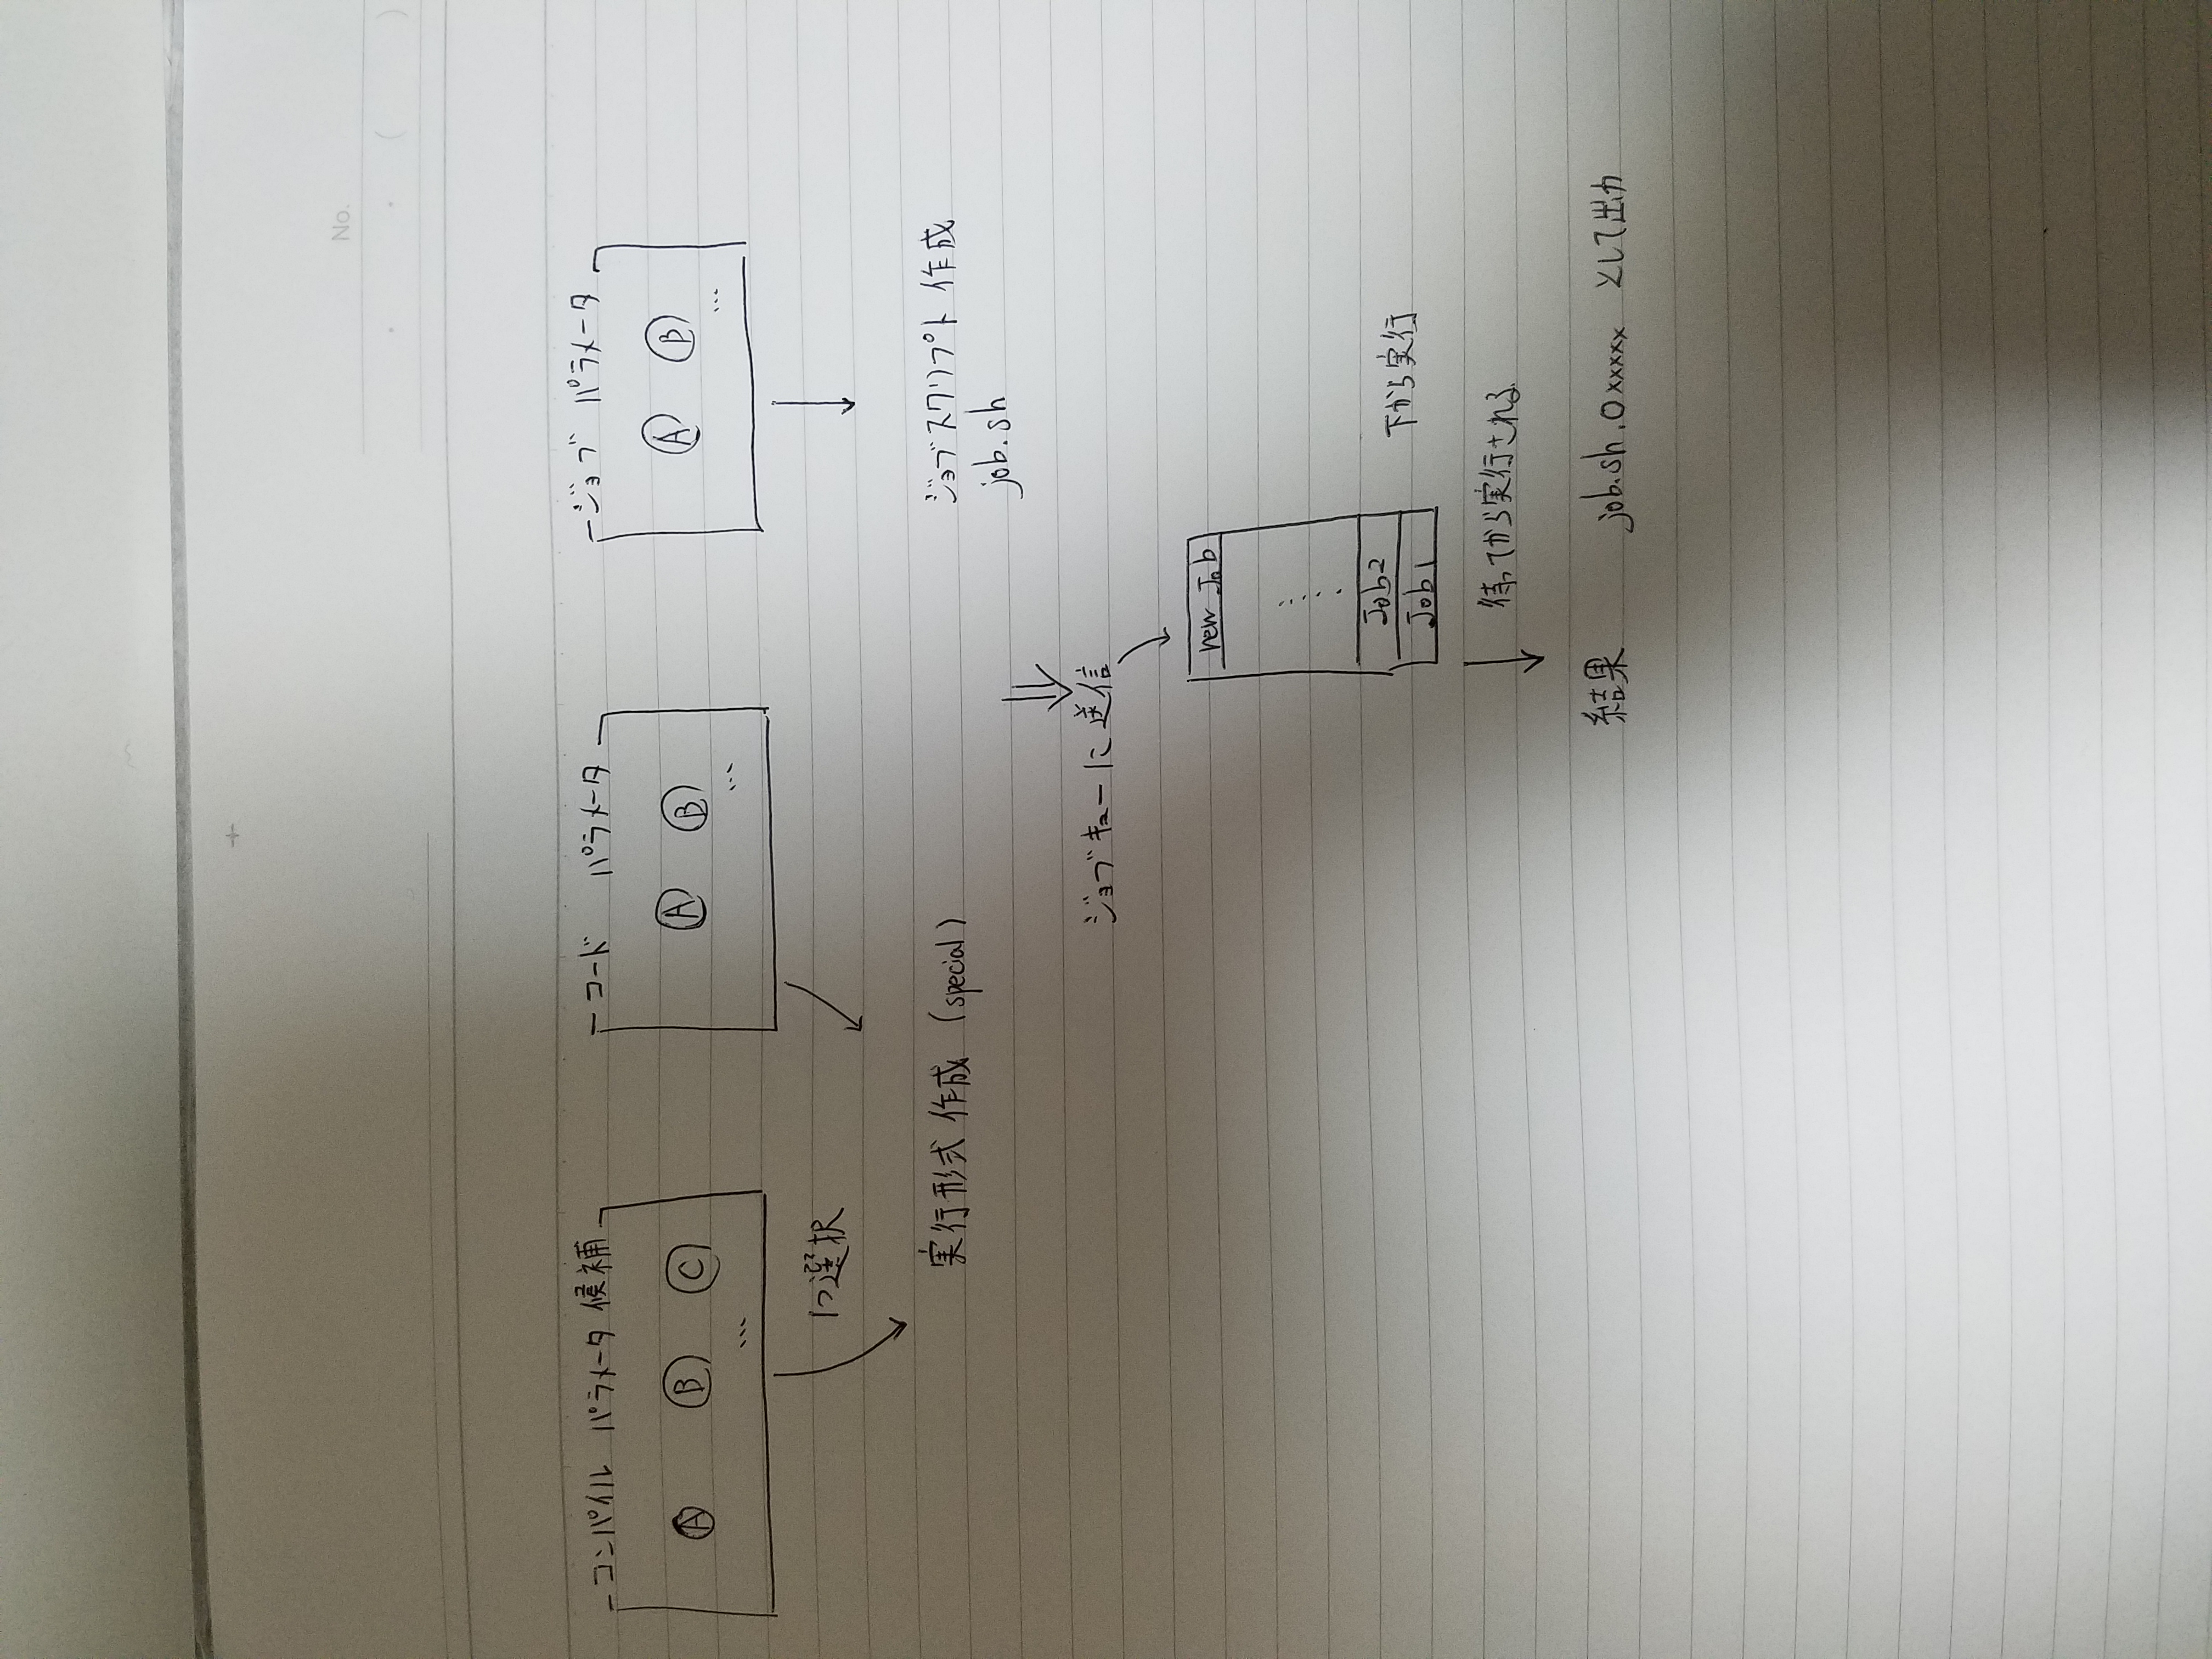
\includegraphics[width=10.0cm]{./images/singlejob}
    \caption{単一ジョブ実行時の挙動}
    \label{fig:singlejob}
  \end{center}
\end{figure}
~\\
図( TODO: 番号)にあるようにジョブの実行はジョブの生成,ジョブの実行,ジョブ結果の集約の3段階に分かれており,
ジョブの生成にかかる時間そしてジョブが実行されるまでのジョブキューでの待機時間がこの一連の動作の実行時間において大きな割合を示す.\\
ジョブが実行されるまでの待機時間は複数のジョブを実行する場合ではジョブの実行時間と同義になるため,これはシミュレーションの内容に応じて変わるが,
ジョブの生成に関してはビルドするプログラムに大きな違いは現れず,多くの場合ジョブの生成時間 $<$ ジョブの実行時間という関係が成立する.\\

また,ジョブの生成部分について詳しく見ると,実行形式とジョブスクリプトそれぞれの生成にかかる時間は表 ( TODO: 表を作る)のようになり,
スーパーコンピュータ京,研究室クラスタ双方において実行形式の生成にかかる時間が多いことがわかる.\\

\paragraph{複数ジョブの並列実行}
次にシミュレータの詳細について複数のジョブの並列実行を例として示す.\\

単一ジョブの実行例からパラメータを選択するためにコード,コンパイル,ジョブそれぞれの候補から一つを選択するという3重のループを組む際に,
最も内側のループ内でジョブスクリプトの生成を行い,外側のループで生成した実行形式を使い回すことでシミュレーションをより高速に行うことができる.\\
また,スーパーコンピュータ京のように非常に多くのノードを持つマシンでない場合,ジョブの実行時間の方が長いため多数のジョブがジョブキューに溜まる状態になる.
そのため,外側のループで実行形式を生成する形を取ることで,ジョブの実行が溜まっているうちに実行形式のビルドを行うことができるようになり,結果として最初の一回を除き以降のビルドは
シミュレーションの実行時間に関与しなくすることができる.\\

本研究では以上を念頭に置きシミュレータのプログラムを作成した.\\
単一ジョブの実行 ( TODO: add ref)で述べたように,ジョブの実行をするにはジョブの生成,ジョブの実行,ジョブ結果の集約が必要となる.\\
その中でジョブの実行はqsubやpjsubといった環境にインストールされているジョブ実行環境を利用するため,シミュレータはジョブの生成と結果の集約の役割を担う.~\\
\begin{figure}[htb]
% h:here, t:top, b:bottom, p:page
  \begin{center}
    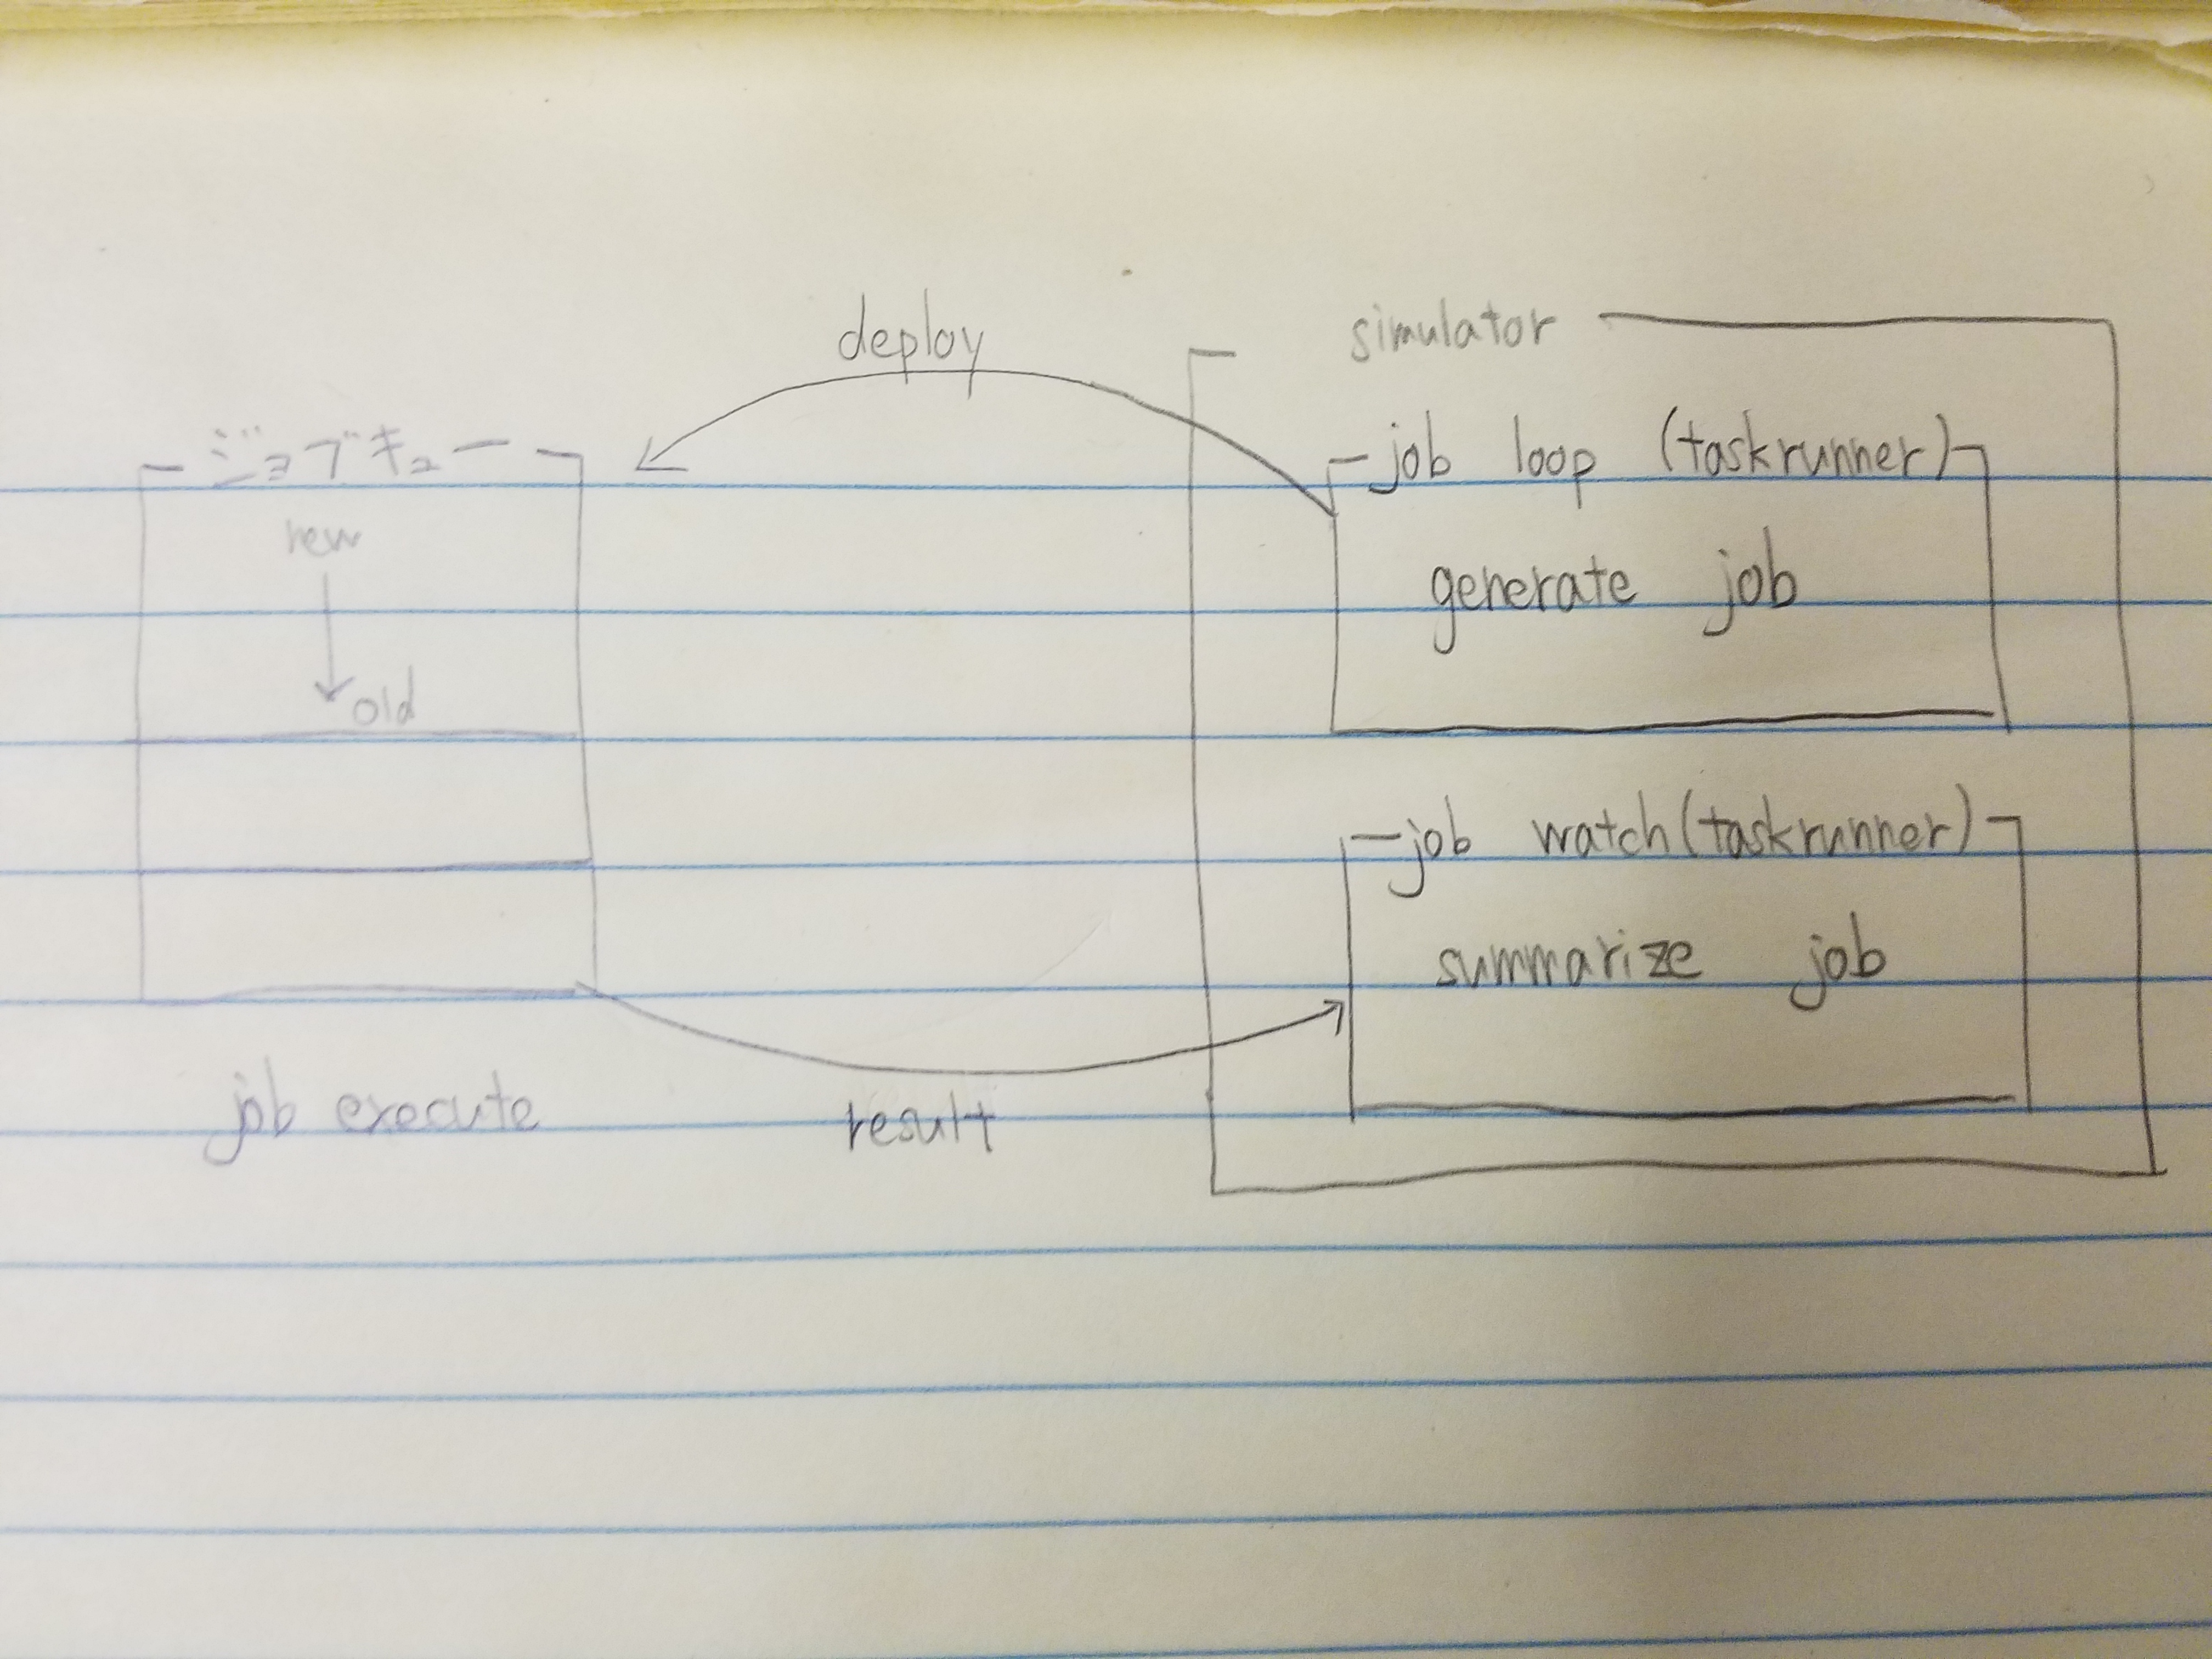
\includegraphics[width=10.0cm, angle=-90]{./images/simulator.pdf}
    \caption{シミュレータ 構成}
    \label{fig:simulator}
  \end{center}
\end{figure}
そのため,シミュレータは次の疑似コードで示す通りジョブを生成するためのループと
メインスレッドから切り離されたスレッドでジョブの実行状況を監視し,
ジョブが終了したタイミングで結果の集約を行うメソッドという二つの機能から成り立っている.~\\
{\footnotesize
\lstinputlisting[caption=シミュレータ疑似コード,label=pseudocode-simulator,frame=single]{src/pseudocode/simulator}
}
上記の疑似コードを状態遷移図の形で可視化したものが次になる.\\
\begin{figure}[htb]
% h:here, t:top, b:bottom, p:page
  \begin{center}
    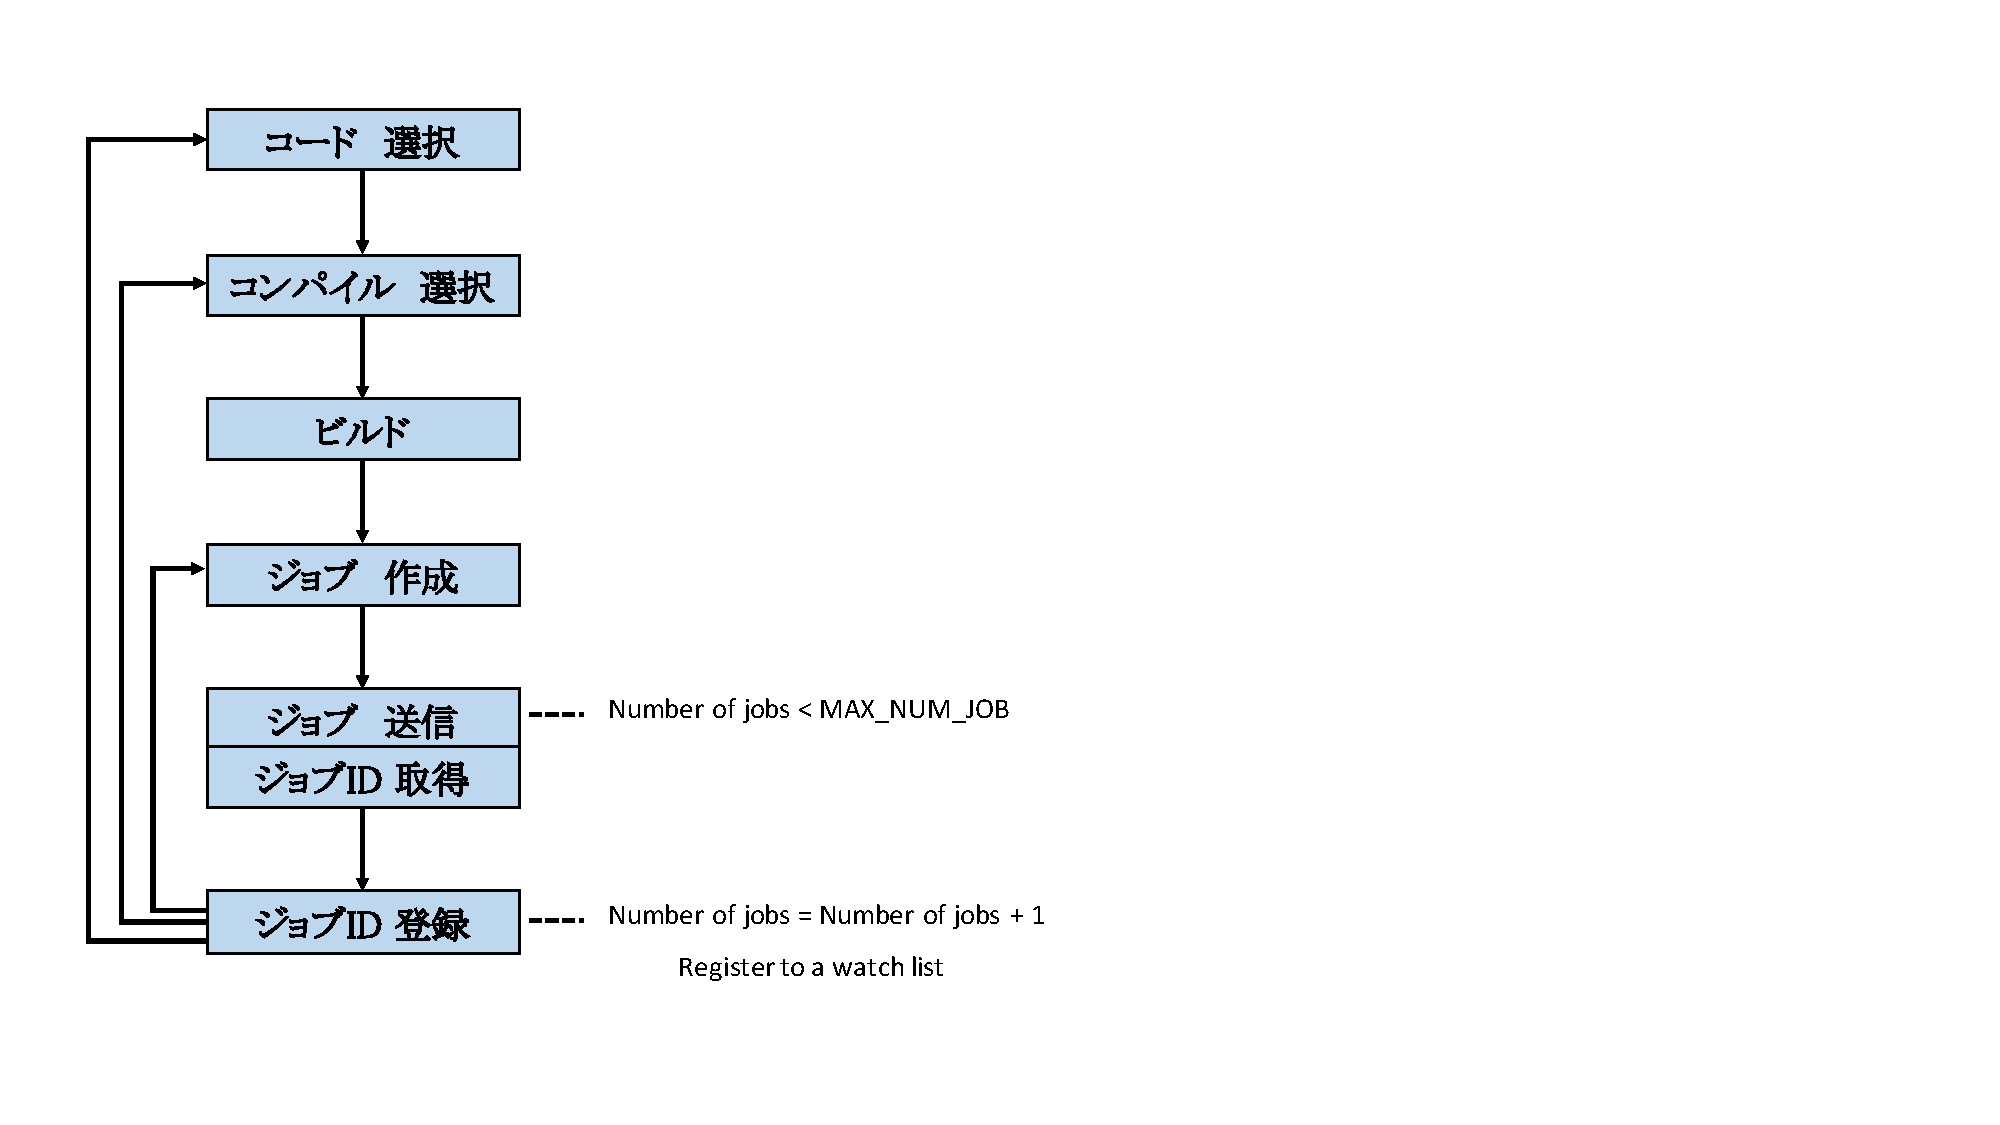
\includegraphics[width=20.0cm]{./images/state.pdf}
    \caption{シミュレータ 状態遷移図}
    \label{fig:simulator-state}
  \end{center}
\end{figure}
~\\
また,環境によってはステージングが存在せず,ジョブキューからジョブが実行される段階になって初めて実行形式とジョブスクリプトにアクセスする
ことになるが,その場合実行形式はそれぞれのビルドごとに,ジョブスクリプトはすべてのジョブに対して区別する必要がある.\\
そのため,実行形式に関してはビルドに関連するディレクトリのコピーをシミュレーションを実行する際に作成し,ビルドごとに参照するディレクトリを切り替え,
ジョブスクリプトに関してはすべてのジョブに対して一意なIDを降りそのIDを元に参照させることにした.\\
( TODO: add 図)
\subparagraph{ジョブ生成ループ}~\\
疑似コード内の8-22行目までがジョブ生成のためのループを構成している.\\
{\footnotesize
\lstinputlisting[caption=シミュレータ ジョブ生成ループ,label=pseudocode-simulator-job-gen-loop,frame=single, firstline=8, lastline=22]{src/pseudocode/simulator}
}
~\\
ループ内部では,プログラムのビルド,ジョブスクリプトの生成,そして生成した実行形式とジョブスクリプトをジョブキューにdeployするという3つのことを行っている.\\
すでに ( TODO: add re)で述べたようにパラメータ候補の選択順を実効形式の生成に関わるものを先にすることで,非同期的に実行形式の生成とジョブの実行を行うことができる.\\
~\\
\subparagraph{ジョブ実行}~\\
{\footnotesize
\lstinputlisting[caption=シミュレータ ジョブ実行,label=pseudocode-simulator-job-deploy,frame=single, firstline=24, lastline=29]{src/pseudocode/simulator}
}
スーパーコンピュータ京のような複数のユーザーが用いるシステムにおいて,ジョブを一度に大量に投げるのは好ましくない.\\
そのため,ジョブをジョブキューに投げる前に事前に設定した最大同時ジョブ実行数と現在の実行中のジョブの数を比較し,最大数と同数なのであれば待機する処理が必要である.\\
本研究では,グローバル変数として現在実行中のジョブのIDを保持するリストを定義し,そのリストの数と比較することで実現している.\\
また,後述するジョブ結果の集約においてこのジョブIDを保持するリストは別スレッドから参照されており,リスト内のジョブが完了した段階でmutexによってロックされた上で更新される.\\
\paragraph{ジョブ結果の集約}~\\
{\footnotesize
\lstinputlisting[caption=シミュレータ ジョブ結果の集約,label=pseudocode-simulator-job-summarize,frame=single, firstline=31, lastline=37]{src/pseudocode/simulator}
}
様々なパラメータの組の中から最適な組み合わせを選びたいため,それぞれのジョブの結果とパラメータの組を結びつける必要がある.\\
先行研究 ( TODO: ref)ではFLOPSを用いて計算性能を測っていたが,そのためにはそれぞれのモデルでシミュレーションを行う際に浮動小数点演算が何回行われるかを
事前または事後的に知る必要がある.\\
しかしながら本研究では,事前情報のない新規のモデルに対しても自動チューニングの対象となるためFLOPSは指標として適さない.
そのため,本研究ではNEURON内での実行時間をシミュレーション内部で終了時に出力させ,指標として用いることにした.\\
{\footnotesize
\lstinputlisting[caption=ベンチマークでNEURON内部での実行時間を出力している箇所,label=neuron-job-script,frame=single]{src/job/time-output-setting}
}
ここでは29行目で出力しているcore timeが実行時間に該当する.\\


ジョブの実行時間のフォーマットは固定されているため,
上記の正規表現を用いて取得することができる.\\
Pythonにおいては,
{\footnotesize
\lstinputlisting[caption=ジョブ実行結果取得,label=get-exec-time,frame=single]{src/python/get-exec-time.py}
}
として取得できる.\\
次に,ジョブが完了しているかの判定を行う方法について述べる.\\
ここではスーパーコンピュータ京と研究室クラスタを例にする.\\
{\footnotesize
\begin{lstlisting}[numbers=none]
京
>> pjstat

研究室クラスタ
>> qstat
Every 1.0s: qstat                                                                                                                                            Wed Jan 10 01:06:06 2018

Job ID                    Name             User            Time Use S Queue
------------------------- ---------------- --------------- -------- - -----
13282.cluster              job223.sh        inoue           00:09:29 C cluster
13283.cluster              job224.sh        inoue           00:04:46 C cluster
13284.cluster              job225.sh        inoue           00:06:48 C cluster
13285.cluster              job226.sh        inoue           00:05:38 C cluster
13286.cluster              job227.sh        inoue           00:05:36 C cluster
13287.cluster              job228.sh        inoue           00:07:16 C cluster
13288.cluster              job229.sh        inoue           00:05:38 C cluster
13289.cluster              job230.sh        inoue           00:07:23 C cluster
13290.cluster              job231.sh        inoue           00:05:37 C cluster
13291.cluster              job232.sh        inoue           00:07:15 C cluster
13292.cluster              job233.sh        inoue           00:05:38 C cluster
13293.cluster              job234.sh        inoue           00:07:16 C cluster
13294.cluster              job235.sh        inoue           00:05:37 C cluster
13295.cluster              job236.sh        inoue           00:07:07 C cluster
13296.cluster              job237.sh        inoue           00:05:35 C cluster
13297.cluster              job238.sh        inoue           00:07:07 C cluster
13298.cluster              job239.sh        inoue           00:05:36 C cluster
13299.cluster              job240.sh        inoue           00:07:08 C cluster
13300.cluster              job241.sh        inoue           00:05:38 C cluster
13301.cluster              job242.sh        inoue                  0 R cluster
\end{lstlisting}
}
京ではpjstat, 研究室クラスタではqstatというコマンドを用いることで現在実行中のジョブを一覧で取得することができる.\\
この中でジョブの状態(State)を表すSの列に注目すると, まだジョブキューの中で実行を待っているQ,実行中のR,実行完了のCのようにジョブの状態を詳細に知ることができることがわかる.\\
また,このコマンドの出力結果も同一のフォーマットに従っているため,正規表現を利用することでジョブの状態を取得することができる.\\
ここではジョブが完了しているか否かの判定を行たいため,
{\footnotesize
\lstinputlisting[caption=ジョブ完了判定,label=is-job-done,frame=single]{src/python/is-job-done.py}
}
とすることでジョブIDを元にジョブの状態を取得することができる.\\

最後に,実際の実行結果が最適化を通して変化していないことの確認も必要である.\\
これは実行結果のファイルを見ることで判断できるが,複数プロセス・スレッドを用いた場合途中の出力結果の順番がランダムになっているという問題があった.\\
ジョブの実行結果は次に示される3つの関数で出力される.\\
{\footnotesize
\lstinputlisting[caption=ジョブ実行結果出力箇所,label=job-output-setting,frame=single]{src/job/output-setting}
}
また,その実行結果を一部抜粋した元が次になる.\\
{\footnotesize
\lstinputlisting[caption=ジョブ実行結果一部抜粋,label=job-output,frame=single]{src/job/output}
}
仮に同じシミュレーションをシングルプロセス・シングルスレッドで行った場合,上記の結果は
{\footnotesize
\lstinputlisting[caption=シングルスレッドで実行する場合の実行結果,label=job-output-sorted,frame=single]{src/job/output-sorted}
}
のようにIDが昇順になる.\\
そのため,実行結果を比較する際には,3種類の関数print\_stat,spikeout,printSpikeStatからの出力結果をそれぞれソートした上で比較する必要がある.\\
本研究においては,出力の形式がそれぞれの関数で固定であり,上記の3種類の関数のみがシミュレーションの実行結果と関係しているため,
IDを元にソートをかけ,ソート後の出力結果を格納した配列のハッシュ値を比較することで実行結果に変化がないことを確かめた.\\
{\footnotesize
\lstinputlisting[caption=実行結果比較コード,label=compare-job-output,frame=single]{src/python/compare-job-output.py}
}
すべてのジョブ結果のファイルに対し,それぞれの行が各関数に該当する正規表現と一致するか調べ,
一致する場合はIDを元にしてならべかえる.\\
並べ替えが終わった段階でhash値を計算し,すべてのファイルに対してhash値が共通のものであるかを確認している.\\
